\subsubsection{الگوی \lr{Heterogeneous Redundancy}}
\label{archSafeHeteroRedundancySec}
\begin{RTL}
الگوی تکرار ناهمگن \cite{ref4}
با استفاده از چندین کانال که به‌طور مستقل طراحی شده‌اند،
تشخیص خطاها را بهبود می‌بخشد و هم خطاهای سیستماتیک و
هم خطاهای تصادفی را شناسایی می‌کند. این الگو به دلیل نیاز بیشتر به زحمت
توسعه و هزینه‌های تکراری، پرهزینه‌تر از
\nameref{archSafeHomoRedundancySec} است. برای
سیستم‌های با ایمنی و قابلیت اطمینان بالا مناسب است
و عملکرد مداوم را حتی در صورت بروز خطاها تضمین می‌کند. با این حال،
هزینه‌های بالا به دلیل نیاز به طراحی‌های مستقل، معمولاً توسط تیم‌های مختلف
به منظور جلوگیری از خطاهای سیستماتیک، ناشی می‌شود. این الگو حفاظت
قوی در برابر خطاها ارائه می‌دهد اما با هزینه بیشتر، و به‌عنوان امن‌ترین اما
پرهزینه‌ترین گزینه معماری در نظر گرفته می‌شود.
ترکیب این الگو با \nameref{archSafeTripModRedunSec} می‌تواند
در دسترس بودن را بیشتر افزایش دهد.
\end{RTL}
\begin{figure}[h!]
\centering
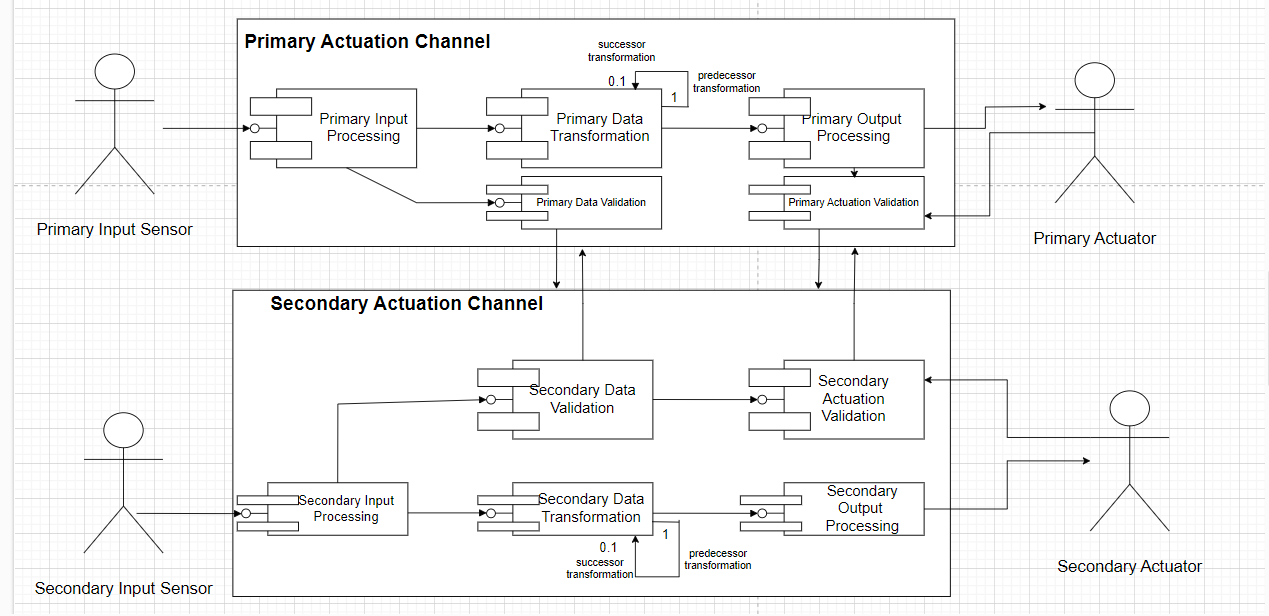
\includegraphics[scale=0.5]{images/second/hetero.png}
\caption{ساختار الگوی \lr{Heterogeneous Redundancy}}
\end{figure}